\documentclass[letterpaper,12pt]{article}
\usepackage{array}
\usepackage{threeparttable}
\usepackage{geometry}
\geometry{letterpaper,tmargin=1in,bmargin=1in,lmargin=1.25in,rmargin=1.25in}
\usepackage{fancyhdr,lastpage}
\pagestyle{fancy}
\lhead{}
\chead{}
\rhead{}
\lfoot{}
\cfoot{}
\rfoot{\footnotesize\textsl{Page \thepage\ of \pageref{LastPage}}}
\renewcommand\headrulewidth{0pt}
\renewcommand\footrulewidth{0pt}
\usepackage[format=hang,font=normalsize,labelfont=bf]{caption}
\usepackage{listings}
\lstset{frame=single,
  language=Python,
  showstringspaces=false,
  columns=flexible,
  basicstyle={\small\ttfamily},
  numbers=none,
  breaklines=true,
  breakatwhitespace=true
  tabsize=3
}
\usepackage{amsmath}
\usepackage{amssymb}
\usepackage{amsthm}
\usepackage{harvard}
\usepackage{setspace}
\usepackage{float,color}
\usepackage[pdftex]{graphicx}
\usepackage{hyperref}
\hypersetup{colorlinks,linkcolor=red,urlcolor=blue}
\theoremstyle{definition}
\newtheorem{theorem}{Theorem}
\newtheorem{acknowledgement}[theorem]{Acknowledgement}
\newtheorem{algorithm}[theorem]{Algorithm}
\newtheorem{axiom}[theorem]{Axiom}
\newtheorem{case}[theorem]{Case}
\newtheorem{claim}[theorem]{Claim}
\newtheorem{conclusion}[theorem]{Conclusion}
\newtheorem{condition}[theorem]{Condition}
\newtheorem{conjecture}[theorem]{Conjecture}
\newtheorem{corollary}[theorem]{Corollary}
\newtheorem{criterion}[theorem]{Criterion}
\newtheorem{definition}[theorem]{Definition}
\newtheorem{derivation}{Derivation} % Number derivations on their own
\newtheorem{example}[theorem]{Example}
\newtheorem{exercise}[theorem]{Exercise}
\newtheorem{lemma}[theorem]{Lemma}
\newtheorem{notation}[theorem]{Notation}
\newtheorem{problem}[theorem]{Problem}
\newtheorem{proposition}{Proposition} % Number propositions on their own
\newtheorem{remark}[theorem]{Remark}
\newtheorem{solution}[theorem]{Solution}
\newtheorem{summary}[theorem]{Summary}
%\numberwithin{equation}{section}
\bibliographystyle{aer}
\newcommand\ve{\varepsilon}
\newcommand\boldline{\arrayrulewidth{1pt}\hline}
\begin{document}

% ----------------------------------------------------------------------
\begin{flushleft}
  \textbf{\large{Problem Set \#2}} \\
  MACS 30100, Dr. Evans \\
  Chih-Yu Chiang \\
  Python Version: 3.5.2
\end{flushleft}
\vspace{5mm}
\noindent\textbf{Problem 1} \\
\noindent\textbf{Part (a). histogram} \\
\\
A histogram of annual incomes of students who graduated in 2018, 2019, and 2020 from the University of Chicago M.A. Program in Computational Social Science. \\
\\
\begin{figure}[htb]\centering\captionsetup{width=6.0in}
  \caption{\textbf{}}
  \fbox{\resizebox{4.0in}{3.0in}{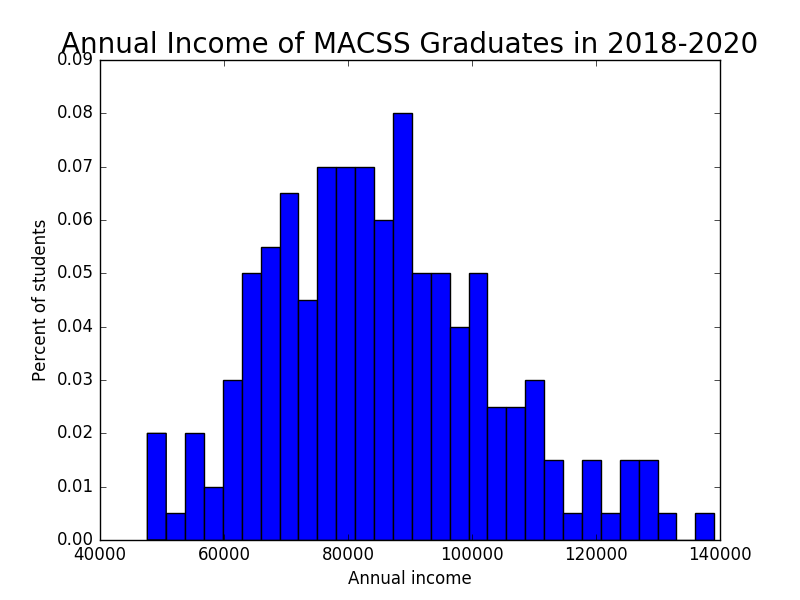
\includegraphics{1a.png}}}
\end{figure} \\

\clearpage

% ----------------------------------------------------------------------
\noindent\textbf{Part (b). log likelihood pdf} \\
\\
A lognormal pdf with $\mu$ = 9.0 and $\sigma$ = 0.3, for 0 $\leq x \leq$ 150,000 is ploted. \\
The log-likelihood value is -8298.636956005032. \\
\\
\begin{figure}[htb]\centering\captionsetup{width=6.0in}
  \caption{\textbf{}}
  \fbox{\resizebox{4.0in}{3.0in}{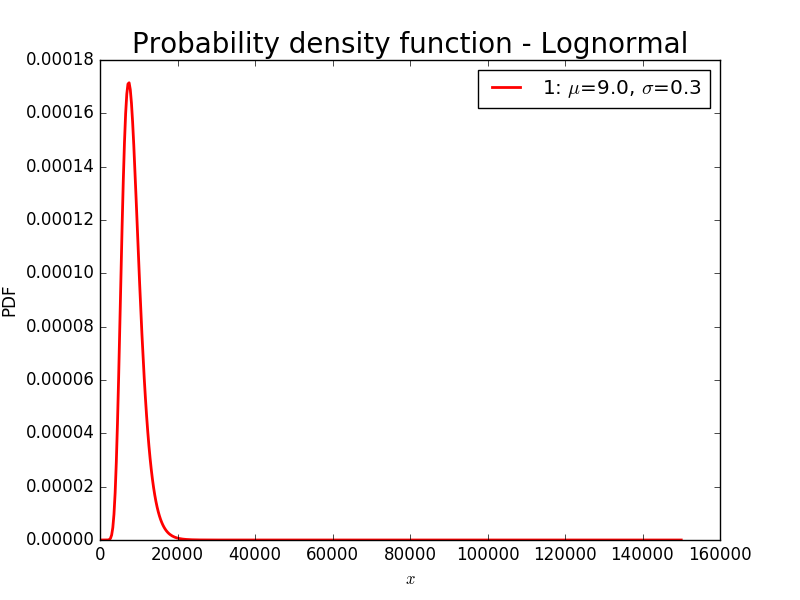
\includegraphics{1b.png}}}
\end{figure} \\

\clearpage

% ----------------------------------------------------------------------
\noindent\textbf{Part (c). estimate distribution} \\
\\
The estimated parameters are as follows: \\
\[\mu_{(MLE)}= 11.3314403048\]
\[\sigma_{(MLE)}= 0.211674604497\]
\\
The maximized log-likelihood is -2239.5347439980105. \\
\[
VCV_{(MLE)} =
\left [
  \begin{tabular}{cc}
  0.01967716 & -0.0024631 \\
  -0.0024631 & 0.00042405 \\
  \end{tabular}
\right ]
\]
\begin{figure}[htb]\centering\captionsetup{width=6.0in}
  \caption{\textbf{}}
  \fbox{\resizebox{4.0in}{3.0in}{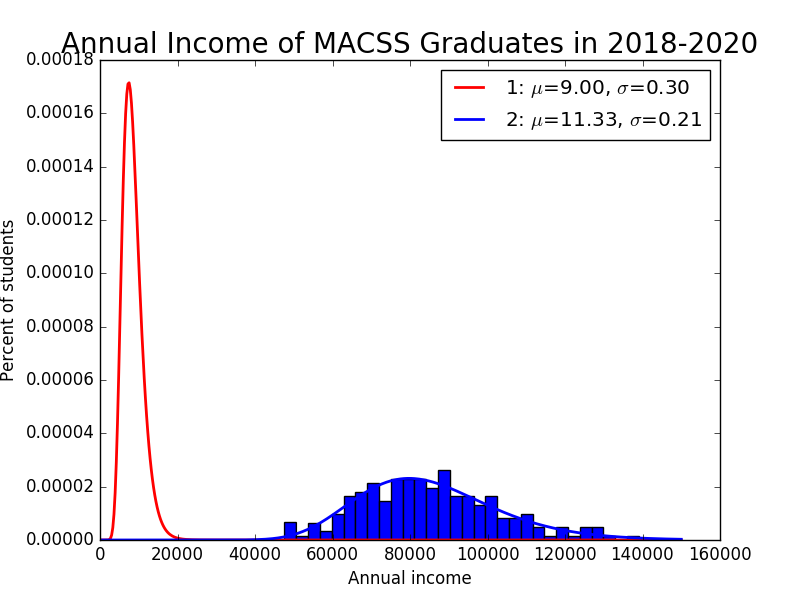
\includegraphics{1c.png}}}
\end{figure} \\

\clearpage

% ----------------------------------------------------------------------

\noindent\textbf{Part (d). chi squared test} \\
\\
$\chi^2$ of $H_0$ with 2 degrees of freedom p-value =  0.0 . \\
That is, the likelihood that the income data came from the distribution is very low.
\\

\noindent\textbf{Part (e). infer proportion} \\
\\
19.58{\%} I will earn more than \$100,000. \\
30.77{\%} I will earn less than \$75,000.
\\
\\
\\
\noindent\textbf{Problem 2} \\
\noindent\textbf{Part (a). estimate linear model} \\
\\
The estimated parameters are as follows: \\
\[\beta_{0(MLE)}= 0.25164631958\]
\[\beta_{1(MLE)}= 0.012933347853\]
\[\beta_{2(MLE)}= 0.400502072911\]
\[\beta_{3(MLE)}= -0.00999167071918\]
\[\sigma_{(MLE)}= 0.00301768213759\]
\\
The maximized log-likelihood is 876.8650464331619. \\
\[
VCV_{(MLE)} =
\left [
  \begin{tabular}{ccccc}
  1 & 0 & 0 & 0 & 0 \\
  0 & 1 & 0 & 0 & 0 \\
  0 & 0 & 1 & 0 & 0 \\
  0 & 0 & 0 & 1 & 0 \\
  0 & 0 & 0 & 0 & 1
  \end{tabular}
\right ]
\]

\noindent\textbf{Part (b). chi squared test} \\
\\
$\chi^2$ of $H_0$ with 5 degrees of freedom p-value =  0.0 . \\
That is, the likelihood that age, number of children, and average winter temperature have no effect on the sick days is very low. \\
\end{document}
